\documentclass[pdf]{beamer}
\mode<presentation>{}
\beamertemplatenavigationsymbolsempty
\usepackage{minted}
\usepackage{tikz}
\usepackage{pgffor} %% gives looping with \foreach
\usepackage[absolute,overlay]{textpos}
\usepackage{lmodern} %% scalable latin characters
\usetikzlibrary{arrows,shapes,backgrounds,decorations.text}
\usepackage{multirow}
\usepackage{ifthen}
\usepackage[utf8]{inputenc}

\title{Information storage and flow}
\subtitle{The central dogma}
\author{Martin Jakt}

\definecolor{mintedBg}{rgb}{0.95, 0.95, 0.95}
\definecolor{blockBg}{rgb}{0.6, 0.6, 0.95}
\definecolor{rnaColor}{rgb}{0, 0.6, 0}
\definecolor{cdsColor}{rgb}{0, 0.4, 0.4}
\definecolor{rnaPol}{rgb}{0.8,0,0.8}
\definecolor{ribosomeCol}{rgb}{0.5,0.5,0.1}
\definecolor{protColor}{rgb}{0.6,0,0.6}
%% colours for nucleotides:
\definecolor{dACol}{rgb}{0.5, 0.5, 0}
\definecolor{dCCol}{rgb}{0.8, 0, 0}
\definecolor{dGCol}{rgb}{0, 0.8, 0}
\definecolor{dTCol}{rgb}{0, 0, 0.8}
    
%% define styles for different codes
\newminted{cpp}{linenos, bgcolor=blockBg, fontsize=\footnotesize}
%% then use \begin{cppcode}
\newminted{c}{linenos, bgcolor=mintedBg, fontsize=\footnotesize}
\newminted{perl}{linenos, bgcolor=mintedBg, fontsize=\footnotesize}

\setlength\parindent{0ex}

%% a command for drawing a ribosome structure
%% as two circles
\newcommand{\riboS}[3][0.8]{
  \draw[fill=ribosomeCol] (#2,#3-#1) circle [radius=#1];
  \draw[fill=ribosomeCol] (#2,#3+#1/1.5) circle [radius=#1/1.5];
}

%% a command to draw a protein at a given location:
\newcommand{\protein}[2]{
  \draw[protColor, line width=1] (#1,#2) to [out=180, in=45] (#1-1.5,#2-1)
  to [out=225, in=270] (#1-0.5,#2-2) to [out=270-180, in=330] (#1-1,#2-1.25)
  to [out=330-180, in=90] (#1-2,#2-1)
  to [out=250, in=180] (#1, #2-2);
  \draw[protColor, line width=4, dotted] (#1,#2) to [out=180, in=45] (#1-1.5,#2-1)
  to [out=225, in=270] (#1-0.5, #2-2) to [out=270-180, in=330] (#1-1, #2-1.25)
  to [out=330-180, in=90] (#1-2, #2-1)
  to [out=250, in=180] (#1, #2-2);
}

%% arguments are : length, width, x, y, nucleotide (A,C,G,T indicated by 1,2,3,4)
\newcommand{\drawBasePair}[5]{
  %% first work out what colors to use
  %% in the absence of any kind of array, I can't think
  %% anything better than..
  \def\tc{dACol}
  \def\bc{dTCol}
  \pgfmathparse{(#5 == 2)?1:0}
  \ifdim\pgfmathresult pt>0pt 
    \def\tc{dCCol}
    \def\bc{dGCol}
  \fi
  \pgfmathparse{(#5 == 3)?1:0}
  \ifdim\pgfmathresult pt>0pt 
    \def\tc{dGCol}
    \def\bc{dCCol}
  \fi
  \pgfmathparse{(#5 == 4)?1:0}
  \ifdim\pgfmathresult pt>0pt 
    \def\tc{dTCol}
    \def\bc{dACol}
  \fi
  
  \draw [-,line width=#2, \tc] (#3,#4) -- (#3,#4-#1);
  \draw [-,line width=#2, \bc] (#3,#4-#1) -- (#3,#4-#1-#1);
}

%% a command to define a subheading
\newcommand\subHeading[1]{
  \par\bigskip {\Large\bfseries#1}\par\smallskip
}

%% to make a fontsize smaller than tiny 
%% this isn't how we should do things, but I can't seem to 
%% find a better way
\makeatletter
\newcommand{\miniscule}{\@setfontsize\miniscule{10}{11}}
\makeatother

%% I detest indentation in footnotes etc, so try this:
\makeatletter
\renewcommand\@makefntext[1]{\noindent\makebox[0em][r]{\@makefnmark}\tiny#1}
\makeatother
%% the makeatletter and makeatother are required to allow me to
%% to change the macro beginning with an @. (though when I call it
%% I don't use the @ ... 


\begin{document}

\begin{frame}
  \titlepage
\end{frame}

\begin{frame}{DNA}
  \begin{itemize}
    \item Very long polymer made up of four different types
          of units (dA, dC, dT, dG).
    \item \emph{Read only} memory that contains the information defining
          the organism.
    \item Double helix made up of two DNA molecules; 
      provides a mechanism for copying.
    \item Maintained from generation to generation.
  \end{itemize}
\end{frame}

\begin{frame}{Nucleotides: the units of DNA}
  \begin{figure}[h]
    \begin{tikzpicture}
      \node at (0,0)
            {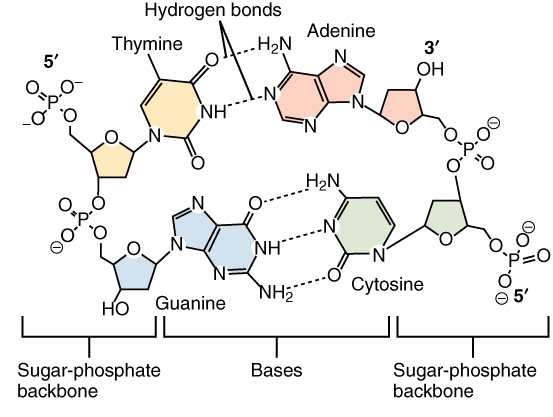
\includegraphics[width=0.5\textwidth]{images/0322_DNA_Nucleotides_crop}};
      \uncover<2->{      
        \draw[red,thick] (-2.22,1.44) circle (0.14cm);
        \draw[red,thick] (1.5,1.59) circle (0.14cm);
      }
    \end{tikzpicture}
  \end{figure}
  \footnotemark
  \footnotetext{ 
    \tiny Image from: "0322 DNA Nucleotides" by OpenStax College - Anatomy \& Physiology, Connexions Web site.\\
    \tiny http://cnx.org/content/col11496/1.6/, Jun 19, 2013.\\
    \tiny Licensed under CC BY 3.0 via Wikimedia Commons\\
    \tiny https://commons.wikimedia.org/wiki/File:0322\_DNA\_Nucleotides.jpg\#/media/File:0322\_DNA\_Nucleotides.jpg
  }
\end{frame}

\begin{frame}{DNA Structure (1)}
  \subHeading{A linear representation}

  \begin{figure}[ht]
    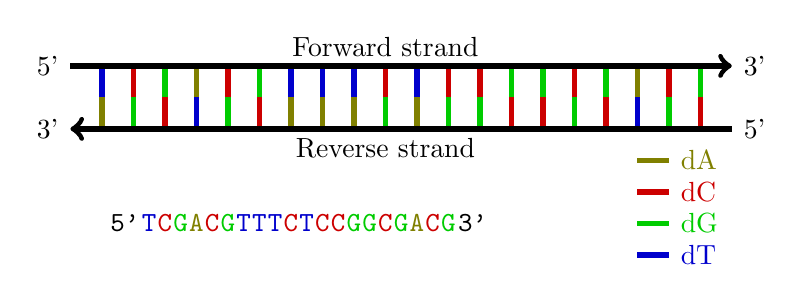
\begin{tikzpicture}[scale=0.4]
      \foreach \i in {1,...,20}{
        \pgfmathsetmacro{\ni}{random(4)};
        \drawBasePair{1}{2}{\i}{3}{\ni};
        \uncover<3->{
          \def\nuc{A} \def\lc{dACol}
          \pgfmathparse{(\ni == 2)?1:0} \ifdim\pgfmathresult pt>0pt \def\nuc{C} \def\lc{dCCol} \fi
          \pgfmathparse{(\ni == 3)?1:0}\ifdim\pgfmathresult pt>0pt \def\nuc{G} \def\lc{dGCol} \fi
          \pgfmathparse{(\ni == 4)?1:0}\ifdim\pgfmathresult pt>0pt \def\nuc{T} \def\lc{dTCol} \fi
          \node [font=\ttfamily, \lc] at (2 + 0.5*\i,-2) {\nuc};
        }
      }
      \draw [->, line width=2] (0,3) node [left] {5'} -- (21,3) node [right] {3'};
      \draw [->, line width=2] (21,1) node [right] {5'} -- (0,1) node [left] {3'};
      \draw [-, line width=2, dACol] (18,0) -- (19,0) node [right] {dA};
      \draw [-, line width=2, dCCol] (18,-1) -- (19,-1) node [right] {dC};
      \draw [-, line width=2, dGCol] (18,-2) -- (19,-2) node [right] {dG};
      \draw [-, line width=2, dTCol] (18,-3) -- (19,-3) node [right] {dT};
      \uncover<2->{
        \node [above] at (10,3) {Forward strand};
        \node [below] at (10,1) {Reverse strand};
      }
      \uncover<3>{
        \node [left, font=\ttfamily] at (2.5,-2) {5'};
        \node [right, font=\ttfamily] at (12,-2) {3'};
      }
    \end{tikzpicture}
  \end{figure}
\end{frame}

\begin{frame}{DNA Structure (2)}
  \begin{figure}[h]
    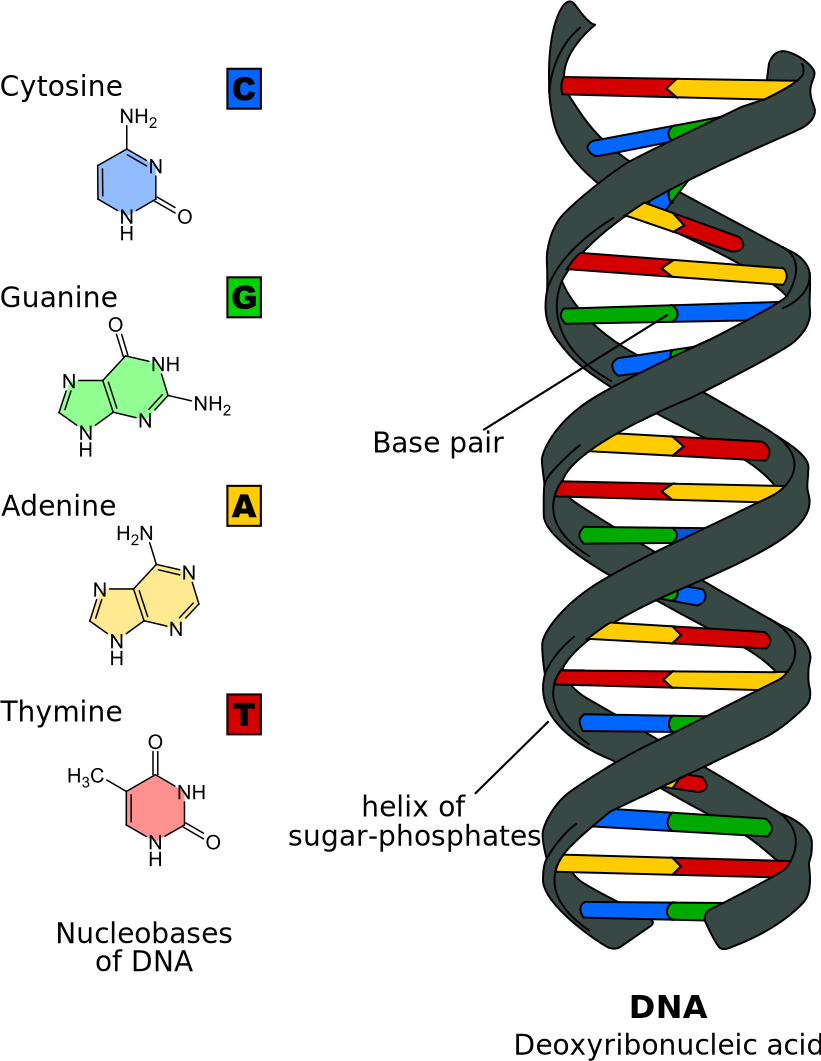
\includegraphics[height=0.75\textheight]{images/DNA}
  \end{figure}
  \tiny Image modified from:\\
  \tiny chemical structures of nucleobases by Roland1952. Licensed under CC BY-SA 3.0 via Wikimedia Commons\\
  \tiny https://commons.wikimedia.org/wiki/File:Difference\_DNA\_RNA-EN.svg
\end{frame}

\begin{frame}{Base pairing to structure}
  \begin{figure}[ht]
    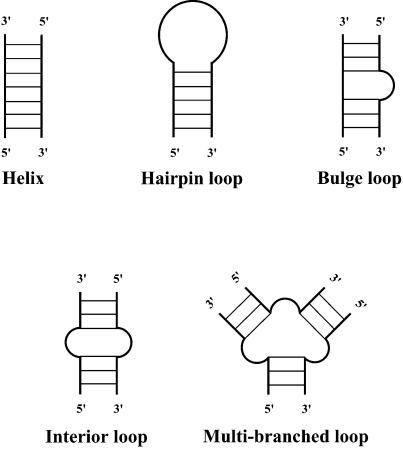
\includegraphics[height=0.7\textheight]{images/oligonucleotide_structures}
  \end{figure}
  \small
  Single stranded RNA / DNA molecules can form complex structures.
  {\tiny
  \\
  Figure 1, from:\\
  Nucleic Acids Res. 2003 Dec 15; 31(24):7280-7301
  \par
  }
\end{frame}

%% The below has been commented out and replaced with the previous frame
%% due to being too complicated to implement within the time frame available
%% and the difficulty of tikz as a general mathematical language
\iffalse
\begin{frame}{Base pairing}
  \begin{figure}[h]
    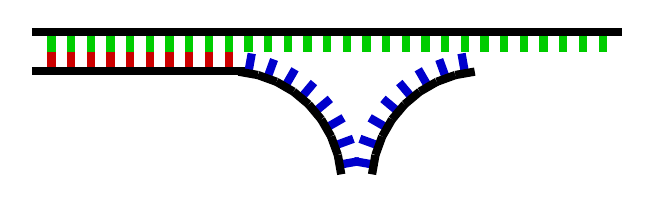
\begin{tikzpicture}[scale=0.5]
%      \draw [help lines] (0, 0) grid (20, 10);
      \foreach \x in {4,4.5,...,18} {
        \draw [-,line width=3, dGCol] (\x,8) -- (\x,7.5);
        \draw [-,line width=3] (\x-0.5,8) -- (\x+0.5,8);
      }
      \foreach \x in {4,4.5,...,8.5} {
        \draw [-,line width=3, dCCol] (\x,7) -- (\x,7.5);
        \draw [-,line width=3] (\x-0.5,7) -- (\x+0.5,7);
      }
      \foreach \a in {80,70,...,10} {
        %% if 10% represents a length of 0.5, then we have
        %% a radius of about 2.87
        %% calculated by (0.25 / sin(5))
        
        \def \x {8.5 + 2.87 * sin(\a)};
        \def \z {15 - 2.87 * sin(\a)};
        \def \y {7-2.87 + 2.87*cos(\a)};
        \def \dx {0.5 * sin(\a)};
        \def \dy {0.5 * cos(\a)};
        \draw [-,line width=3, dTCol] ({\x}, {\y}) -- ({\x+\dx}, {\y+\dy});
        \draw [-,line width=3, dTCol] ({\z}, {\y}) -- ({\z-\dx}, {\y+\dy});
        %% to draw the line calculate..
        \draw [-,line width=3] ({8.5 + 2.87 * sin(\a-5)}, {7-2.87 + 2.87*cos(\a-5)} )
        -- ({8.5 + 2.87 * sin(\a+5)}, {7-2.87 + 2.87*cos(\a+5)} );
        \draw [-,line width=3] ({15 - 2.87 * sin(\a-5)}, {7-2.87 + 2.87*cos(\a-5)} )
        -- ({15 - 2.87 * sin(\a+5)}, {7-2.87 + 2.87*cos(\a+5)} );
      }
    \end{tikzpicture}
  \end{figure}
\end{frame}
\fi

\begin{frame}{Copying DNA}
  \begin{columns}
    \begin{column}{0.3\textwidth}
      \begin{figure}[hb]
        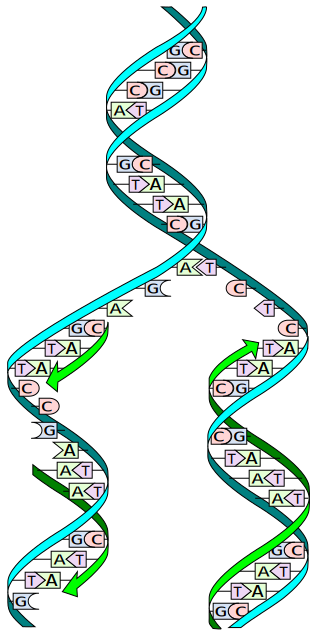
\includegraphics[width=0.8\textwidth]{images/DNA_replication_split}
        %%\caption{DNA Replication\protect\footnotemark}
        %%"DNA replication split" by I, Madprime.}
          %%Licensed under CC BY-SA 3.0 via Wikimedia Commons\\ 
         %% https://commons.wikimedia.org/wiki/File:DNA_replication_split.svg#/media/File:DNA\_replication\_split.svg
      \end{figure}
      \footnotemark
    \end{column}
    \pause
    \begin{column}{0.7\textwidth}
      \begin{figure}[hb]
        \includegraphics[width=0.8\textwidth]{images/Replication_fork}
      \end{figure}
      \footnotemark
    \end{column}
  \end{columns}
  \footnotetext[1]{\tiny https://commons.wikimedia.org/wiki/File:DNA\_Replication\_split.svg }
  \footnotetext[2]{\tiny https://commons.wikimedia.org/wiki/File:Replication\_fork.svg} 
\end{frame}

\begin{frame}{Packaging of DNA in the Nucleus}
  \begin{columns}
    \begin{column}{0.35\textwidth}
      \footnotesize{
        \\
        1 bp $\sim$0.34nm\\
        $6 \times 10^9$ bp / diploid genome\\
        $\sim$2m
      }
    \end{column}
    \begin{column}{0.65\textwidth}
      \begin{figure}[ht]
        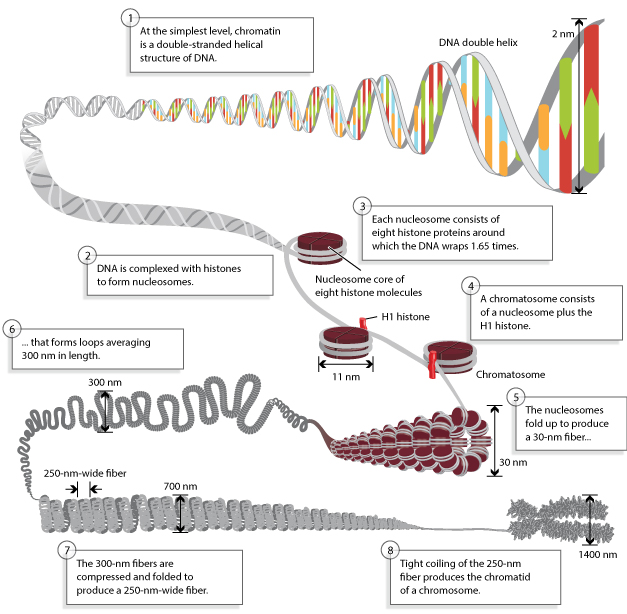
\includegraphics[width=\textwidth]{images/DNA_chromatin}
      \end{figure}
    \end{column}
  \end{columns}
  {\tiny 
  \linespread{0.5}
  DNA Packaging: Nucleosomes and Chromatin\\
  Anthony T. Annunziato, Ph.D. (Biology Department, Boston College) © 2008 Nature Education 
  http://www.nature.com/scitable/topicpage/dna-packaging-nucleosomes-and-chromatin-310
  \par
  }
\end{frame}

\begin{frame}{Packaging and gene regulation}
  \begin{itemize}
  \item Histones can be modified by methylation, acetylation, sumoylation,
    phosphorylation, biotinilation, ubiquitination at specific
    residues.
  \item Specific modifications are correlated with:
    \begin{itemize}
    \item Active transcription
    \item Repressed state
    \item Gene features and their states (eg. promoters / enhancers / splice
      sites(?))
    \end{itemize}
  \item Histone modifications both set and read by transcription factors.
  \item Large number ($\sim$70) of histone modifications known with a
    potentially huge combinatorial code.
  \item Specific histone modifications are also associated with DNA methylation.
  \end{itemize}
  {\tiny For more details:\\
    \url{https://www.cellsignal.com/common/content/content.jsp?id=science-tables-histone}\\
    \url{http://www.activemotif.com/documents/1815.pdf}\\
  }
\end{frame}

%\begin{frame}{Chromosomes}
%  Chromosomes; linear vs circular.

%  Why multiple chromosomes? 
%\end{frame}


\begin{frame}[fragile]{The informatician's representation}
  \begin{columns}
    \begin{column}{0.5\textwidth}
       \begin{verbatim}
ACTGATAGA
|||||||||
TGACTATCT
       \end{verbatim}
    \end{column}
    \begin{column}{0.5\textwidth}
      \uncover<2->{
        or more simply as:
        \begin{semiverbatim}
          \uncover<2->{
            5' ACTGATAGA 3'
          }
        \end{semiverbatim}
        }
    \end{column}
  \end{columns}
  \begin{textblock*}{\textwidth-1em}(0em, \textheight-10ex)
    \raggedleft
    \uncover<3->{
      Simply the sequence of the nucleotides\\
      For human about $3\times10^9$ letters.
    }
  \end{textblock*}  
\end{frame}

\begin{frame}{How to read DNA sequence}
\subHeading{The Gene}
\begin{itemize}
  \item A functional unit of DNA.
  \item Contains a region that is transcribed into RNA
    and encodes the amino acid sequence of a protein or a functional RNA molecule.
  \item Includes the regions that determine when the
    gene is active (RNA is transcribed).
\end{itemize}
As always, this is a bit of an over-simplification.

\end{frame}

\begin{frame}{RNA}
  \subHeading{What is RNA?}
  \begin{itemize}
    \item Like DNA but made up of (A, C, U, G)
    \item Chemically very similar to the DNA but less stable
    \item The units contain three of the same bases as DNA and
      can base-pair with DNA molecules (forming hybrid double stranded molecules).
    \item Uracil (U) base instead of T found in
      DNA molecules. Functionally equivalent and can base pair with A.
    \item RNA molecules transmit genetic information from the DNA, and are used
      either as functional RNA molecules or to encode protein structures.
  \end{itemize}
\end{frame}

\begin{frame}{DNA and RNA monomers}
  \begin{figure}[ht]
    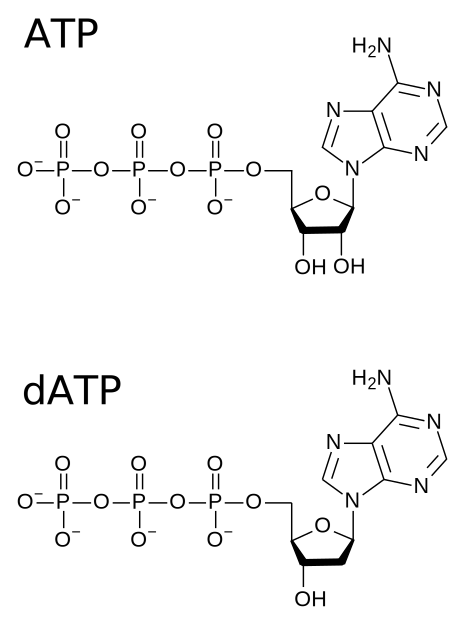
\includegraphics[height=0.7\textheight]{images/ATP_dATP}
  \end{figure}
  Spot the difference!

  {\tiny
    image modified from:\\
    http://www.wikidoc.org/index.php/Nucleotide
    \par
  }
\end{frame}

\begin{frame}{DNA \& RNA structure}
  \begin{figure}[ht]
    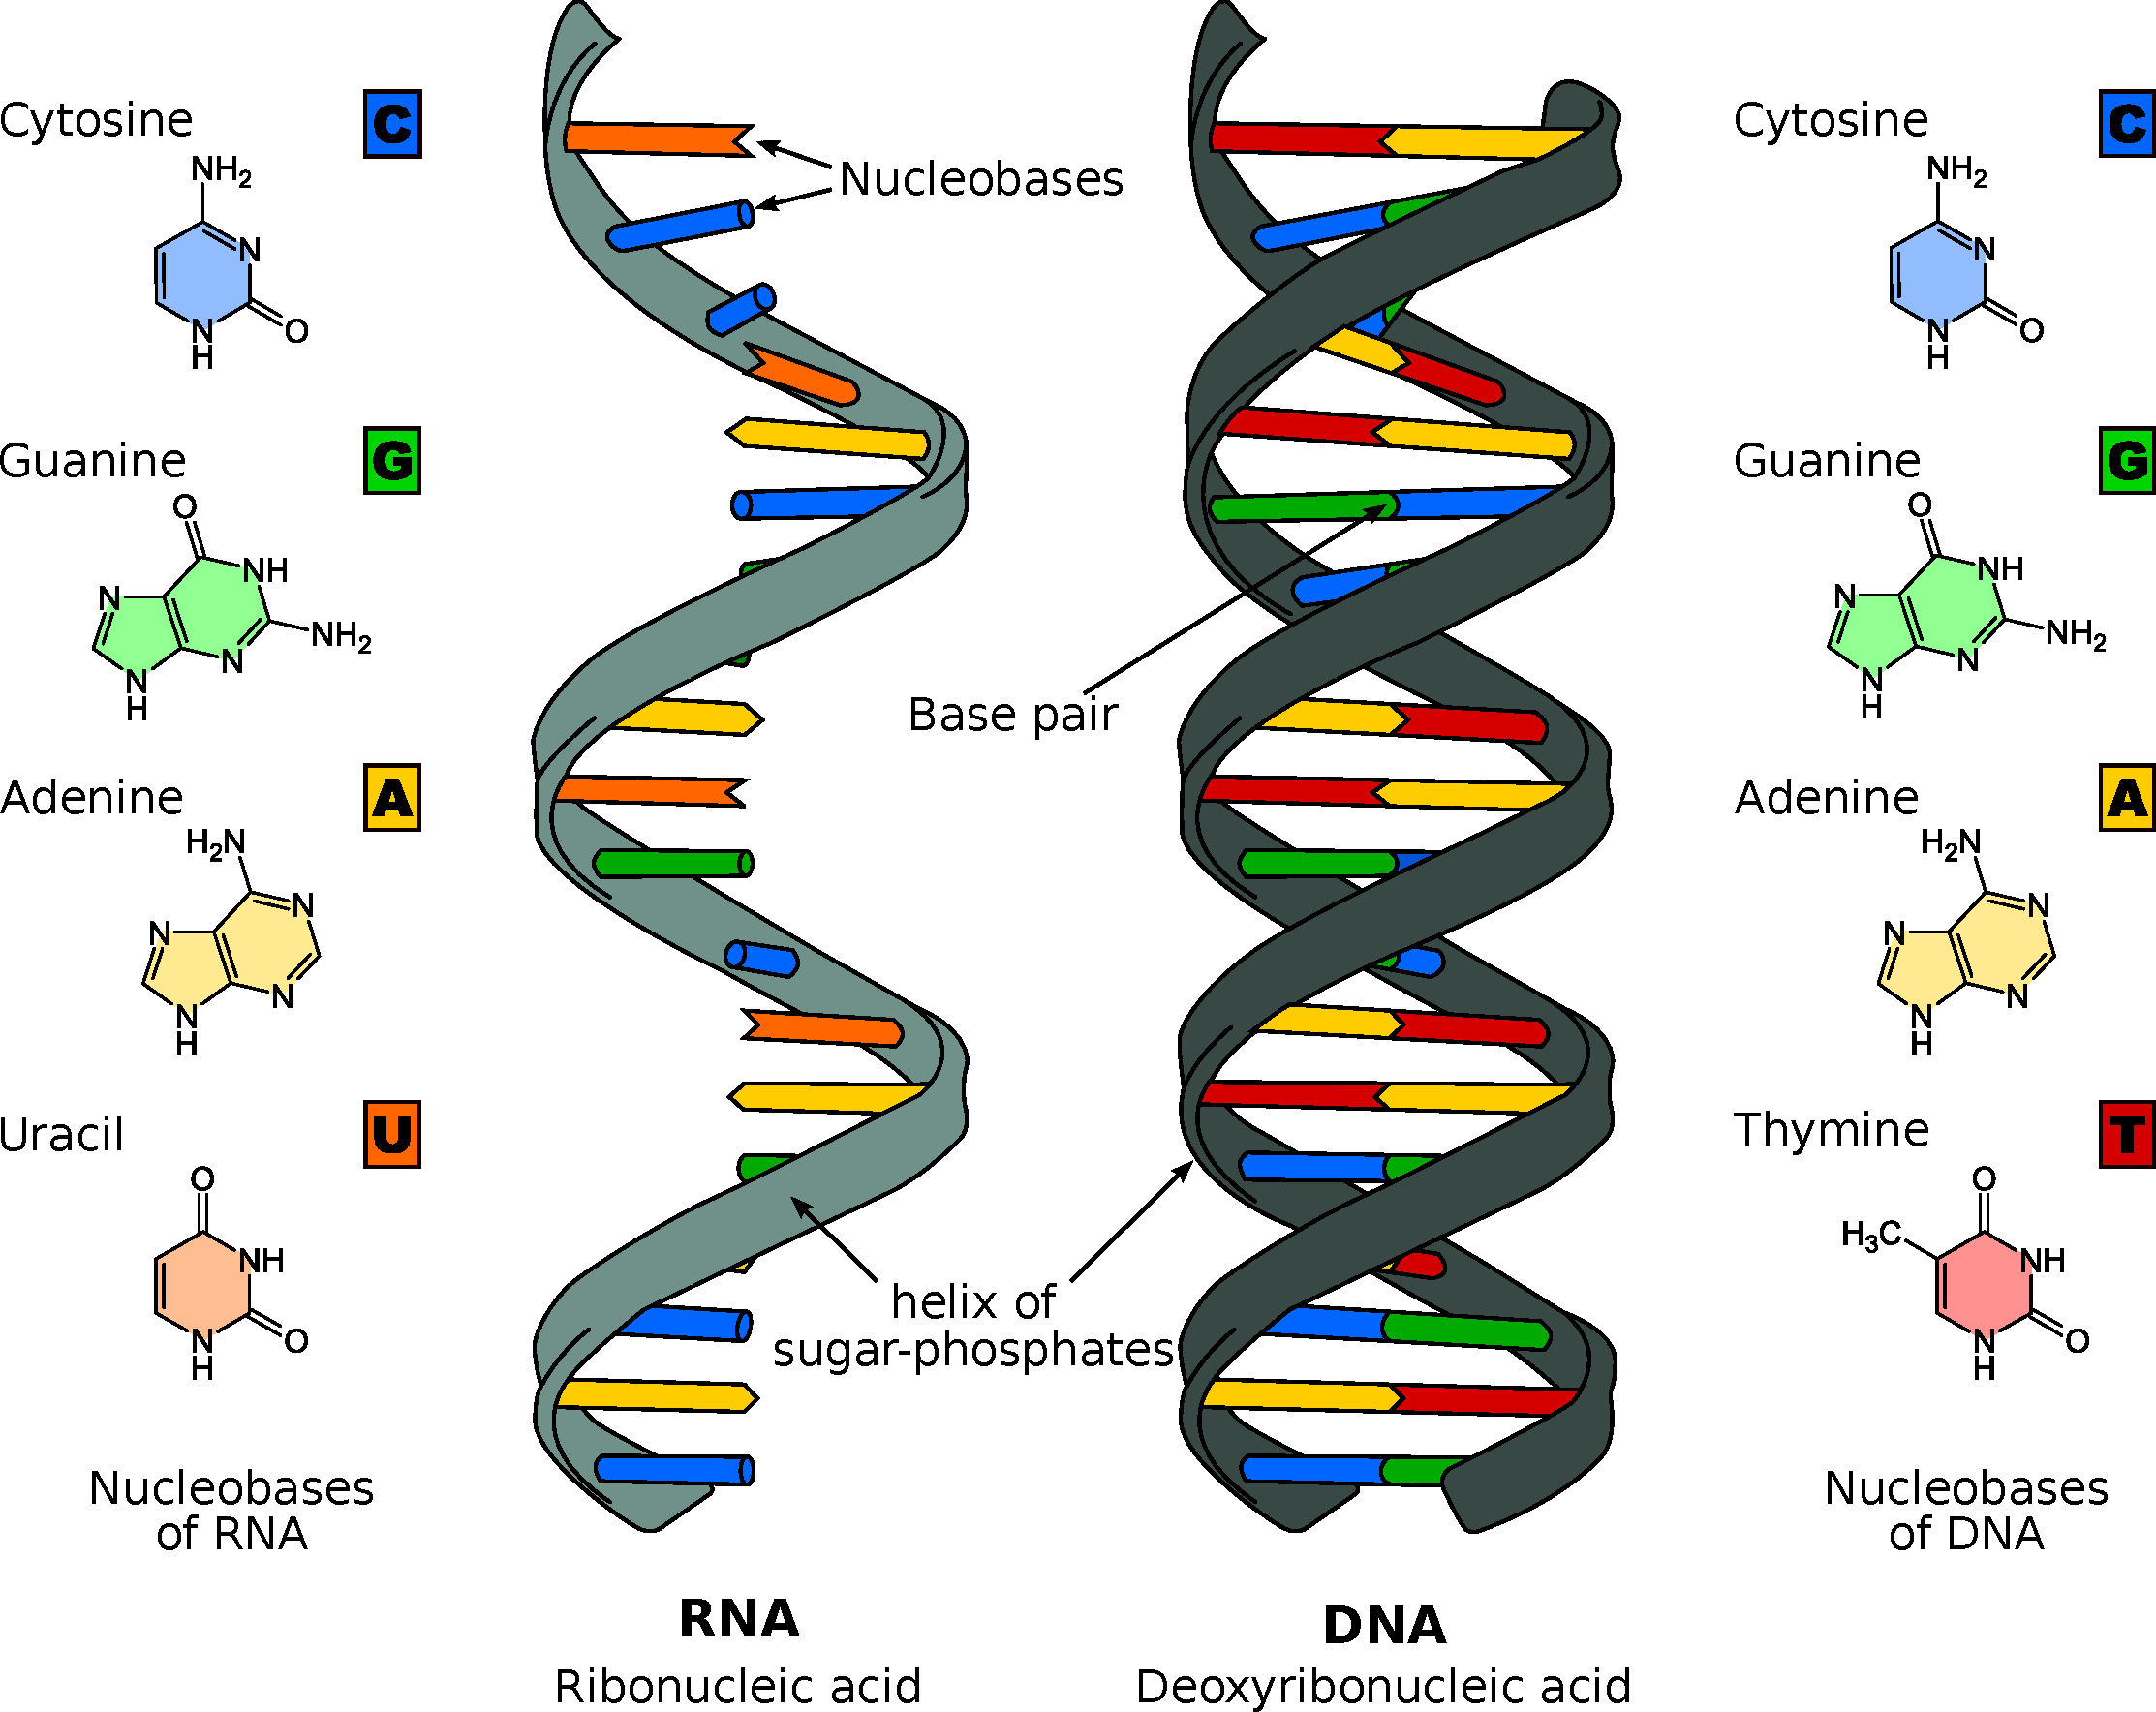
\includegraphics[height=0.7\textheight]{images/Difference_DNA_RNA-EN.pdf}
  \end{figure}
  \small RNA can also be double stranded.

  {\tiny
    image from:\\
    chemical structures of nucleobases by Roland1952. Licensed under CC BY-SA 3.0 via Wikimedia Commons\\
    https://commons.wikimedia.org/wiki/File:Difference\_DNA\_RNA-EN.svg
    \par
  }
\end{frame}

\iffalse
\begin{frame}{RNA-DNA base pairing}
  Very useful for many purposes, including visualising RNA molecules.
  
  Include a picture of FISH and see if they can understand how it is
  achieved.
\end{frame}
\fi

\begin{frame}{Protein}
  \subHeading{What is Protein?}
  \begin{itemize}
    \item Polymer molecules made up of chains of 20 different amino acids.
    \item Make up both structural (e.g. cytoskeleton) and functional (eg. enzymes)
      components of the cells.
    \item Can form an almost infinite variety of shapes that are determined by
      their amino acid sequence (primary structure).
    \item The amino acid sequence determines how the protein molecule folds into
      specific shape and also it's chemical properties.
  \end{itemize}
\end{frame}

\begin{frame}{Amino Acids}
  \begin{figure}[ht]
    \includegraphics[width=0.85\textwidth]{images/Amino_Acids}
  \end{figure}
  {\tiny
    Image elements taken from:\\
    https://en.wikipedia.org/wiki/Genetic\_code\#/media/File:GeneticCode21-version-2.svg\\
    originally by Abgent.
    \par
  }
\end{frame}

\begin{frame}{The Central Dogma}
\begin{figure}[ht]
  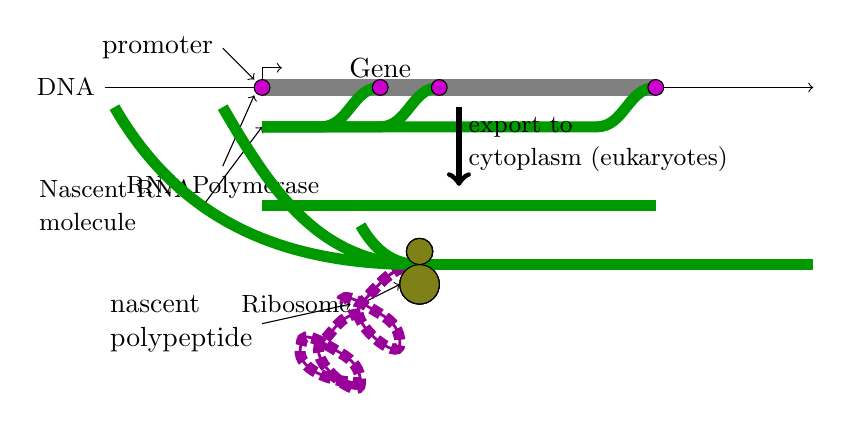
\begin{tikzpicture}[scale=0.5]
%    \draw [help lines] (0,0) grid (20,10);
    \draw [->, black!100] (1,9) -- (19,9);
    \visible<1-1>{ \node [left] at (1,9) {\small DNA}; }
    \uncover<2->{
      \draw[black!50, line width=6] (5,9) -- (15,9);
      \draw[->] (5,9) -- (5,9.5) -- (5.5,9.5);
      \node [above] at (8,9) {Gene};
    }
    
    \visible<3-3>{
%%      \draw[rnaColor, line width=4] (5,8) -- (8,8) 
%%      to [out=0, in=180] (9.5,9);
      \draw [fill=rnaPol] (5,9) circle [radius=0.2];
      \draw [<-] (4.8,8.8) -- (4,7) node[below]
            {\small RNA Polymerase};
      \draw [->] (4,10) node [left] {promoter} -- (4.8,9.2);
    }

    \visible<4-4>{
      \draw[rnaColor, line width=4] (5,8) -- (6.5,8) 
      to [out=0, in=180] (8,9);
      \draw[<-] (5,8) -- (3.5,6) node[left, align=left]
           {\small Nascent RNA\\\small molecule};
      \draw [fill=rnaPol] (8,9) circle [radius=0.2];
    }

    \visible<5-5>{
      \draw[rnaColor, line width=4] (5,8) -- (8,8) 
      to [out=0, in=180] (9.5,9);
      \draw [fill=rnaPol] (9.5,9) circle [radius=0.2];
    }

    \visible<6-6>{
      \draw[rnaColor, line width=4] (5,8) -- (13.5,8) 
      to [out=0, in=180] (15,9);
      \draw [fill=rnaPol] (15,9) circle [radius=0.2];
    }

    \visible<7-7>{
      \draw[rnaColor, line width=4] (5,6) -- (15,6);
      \draw[->, line width=2]  (10,8.5) -- (10,6.5);
      %% node can also take an optional scale= command 
      %% to change font sizes
      \node [below right, align=left] at (10,8.5) 
            {\small export to\\\small cytoplasm (eukaryotes)};
%%      \draw [fill=rnaPol] (15,9) circle [radius=0.2];
    }

    \visible<8-8>{
      \draw[rnaColor, line width=4] (9,4.5) -- (19,4.5);
      \riboS[0.5]{9}{4.5}
      \draw [->] (7.5,3.5) node[left]{\small Ribosome} -- (8.5,4);
    }

    \visible<9-9>{
      \draw[rnaColor, line width=4] (9,4.5) -- (17,4.5);
      \draw[rnaColor, line width=4] (9,4.5) to [out=180, in=300] (7.5,5.5);
      \draw[protColor, line width=1] (9,4.5) to [out=180, in=45] (7.5,3.5);
      \draw[protColor, line width=4, dotted] (9,4.5) to [out=180, in=45] (7.5,3.5);
      \draw [->] (5, 3) node[left, align=left]{nascent\\polypeptide} -- (7.25, 3.5);
      \riboS[0.5]{9}{4.5}
    }

    \visible<10-10>{
      \draw[rnaColor, line width=4] (9,4.5) -- (12,4.5);
      \draw[rnaColor, line width=4] (9,4.5) to [out=180, in=300] (4,8.5);
      \draw[protColor, line width=1] (9,4.5) to [out=180, in=45] (7.5,3.5)
      to [out=225, in=270] (8.5,2.5) to [out=270-180, in=330] (8,3.25)
      to [out=330-180, in=90] (7,3.5);
      \draw[protColor, line width=4, dotted] (9,4.5) to [out=180, in=45] (7.5,3.5)
            to [out=225, in=270] (8.5,2.5) to [out=270-180, in=330] (8,3.25)
            to [out=330-180, in=90] (7,3.5);
      \riboS[0.5]{9}{4.5}
    }

    \visible<11-11>{
      \draw[rnaColor, line width=4] (9,4.5) -- (9.25,4.5);
      \draw[rnaColor, line width=4] (9,4.5) to [out=180, in=300] (1.25,8.5);
      %% the shift and rotate can be put directly into the \draw
      %% command, but as I have two draw commands, using scope is nice
      %% \draw[shift={(1,1)},rotate=20] ...
      \begin{scope}[shift={(-1, -1)},rotate=0]
        \draw[protColor, line width=1] (8.5,4.25) to [out=180, in=45] (7.5,3.5)
        to [out=225, in=270] (8.5,2.5) to [out=270-180, in=330] (8,3.25)
        to [out=330-180, in=90] (7,3.5)
        to [out=250, in=180] (8.5,2.5);
        \draw[protColor, line width=4, dotted] (8.5,4.25) to [out=180, in=45] (7.5,3.5)
        to [out=225, in=270] (8.5,2.5) to [out=270-180, in=330] (8,3.25)
        to [out=330-180, in=90] (7,3.5)
        to [out=250, in=180] (8.5,2.5);
      \end{scope}
      \riboS[0.5]{9}{4.5}
    }

  \end{tikzpicture}
\end{figure}
\end{frame}

\begin{frame}{The Central Dogma}
  \begin{figure}[ht]
    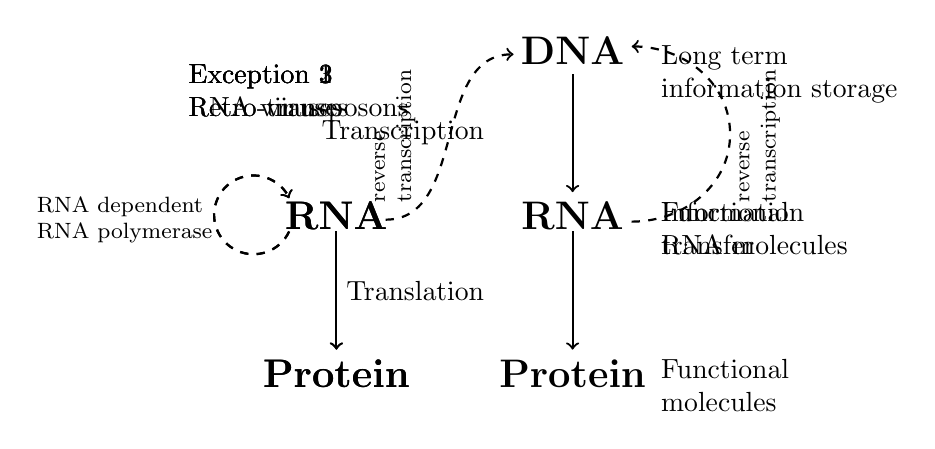
\begin{tikzpicture}[scale=0.5]
%      \draw [help lines] (0,0) grid (20,10);
      \node [above] at (10,9.5) {\Large\bfseries DNA};
      \draw [->,thick] (10,9.5) -- (10,6.5) node [below] {\Large\bfseries RNA};
      \visible<1-4,6->{ \draw [->,thick] (10,5.5) -- (10,2.5) node [below] {\Large\bfseries Protein}; }
      \visible<2-4>{ \node [left] at (8,8) {Transcription}; }
      \visible<3-4>{ \node [left] at (8,4) {Translation}; }
      \visible<4>{
        \node [right, align=left] at (12,9.5) {Long term\\information storage};
        \node [below right, align=left] at (12,6.5) {Information\\transfer};
        \node [below right, align=left] at (12,2.5) {Functional\\molecules};
      }
      \visible<5>{
        \node [below right, align=left] at (0,10) {Exception 1};
        \node [below right, align=left] at (12,6.5) {Functional\\RNA molecules};
      }
      \visible<6>{
        \node [below right, align=left] at (0,10) {Exception 2\\RNA viruses};
        \node [below] at (4,6.5) {\Large\bfseries RNA};
        \draw [->,thick] (4,5.5) -- (4,2.5) node [below] {\Large\bfseries Protein};
        \draw [->,thick,dashed] (2.8,5.5) arc [radius=1, start angle=335,
        end angle=25];
        \node [left, align=left, font=\footnotesize] at (1.1,5.8) {RNA dependent\\RNA polymerase};
      }
      \visible<7>{
        \node [below right, align=left] at (0,10) {Exception 3\\Retro viruses};
        \node [below] at (4,6.5) {\Large\bfseries RNA};
        \draw [->,thick] (4,5.5) -- (4,2.5) node [below] {\Large\bfseries Protein};
        \draw [->,thick,dashed] (2.8,5.5) arc [radius=1, start angle=335,
          end angle=25];
        \draw [->,thick,dashed] (5.25,5.8) to [out=0, in=180] (8.5,10);
        \node [right,align=left,rotate=90, font=\footnotesize ] at (5.5,6) {reverse\\transcription};
      }
      \visible<8>{
        \node [below right, align=left] at (0,10) {Exception 3\\Retro-transposons};
        \draw [->,thick,dashed] (11.5,5.75) to [out=0,in=270] (14,7.975)
        to [out=90,in=0] (11.5,10.2);
        \node [below right,align=left,rotate=90, font=\footnotesize ] at (14,6) {reverse\\transcription};
      }

    \end{tikzpicture}
  \end{figure}
\end{frame}

\begin{frame}{Genes in prokaryotes}
  \subHeading{Operons and polycistronic messages}
  \begin{figure}[ht]
  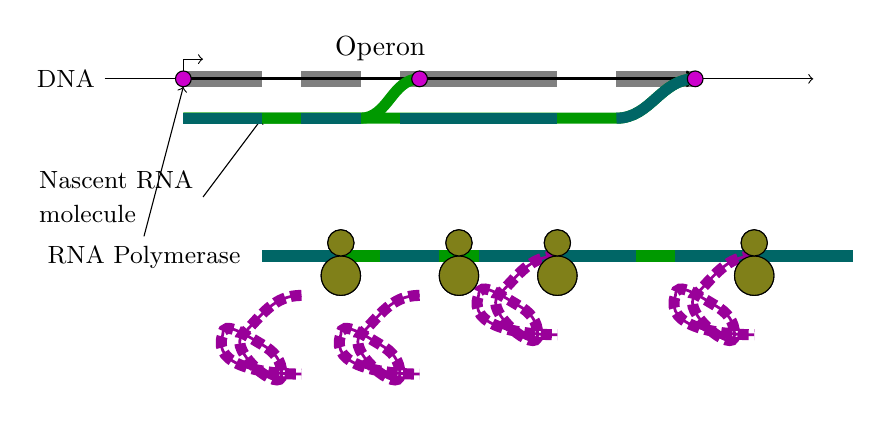
\begin{tikzpicture}[scale=0.5]
%    \draw [help lines] (0,0) grid (20,10);
    \draw [->, black!100] (1,9) -- (19,9);
    \visible<1-1>{ \node [left] at (1,9) {\small DNA}; }
    \uncover<2->{
      \draw[black!50, line width=6] (3,9) -- (5,9);
      \draw[black!50, line width=6] (6,9) -- (7.5,9);
      \draw[black!50, line width=6] (8.5,9) -- (12.5,9);
      \draw[black!50, line width=6] (14,9) -- (16,9);
      \draw[->] (3,9) -- (3,9.5) -- (3.5,9.5);
      \draw[->,line width=1.2] (3,9) -- (16,9);
      \node [above] at (8,9.2) {Operon};
    }
    
    \visible<3-3>{
%%      \draw[rnaColor, line width=4] (5,8) -- (8,8) 
%%      to [out=0, in=180] (9.5,9);
      \draw [fill=rnaPol] (3,9) circle [radius=0.2];
      \draw [<-] (3,8.8) -- (2,5) node[below]
            {\small RNA Polymerase};
    }

    \visible<4-4>{
      \draw[rnaColor, line width=4] (3,8) -- (7.5,8) 
      to [out=0, in=180] (9,9);
      \draw[cdsColor, line width=4] (3,8) -- (5,8);
      \draw[cdsColor, line width=4] (6,8) -- (7.5,8);
      \draw[<-] (5,8) -- (3.5,6) node[left, align=left] {\small Nascent RNA\\\small molecule};
          
      \draw [fill=rnaPol] (9,9) circle [radius=0.2];
    }

    \visible<5-5>{
      \draw[rnaColor, line width=4] (3,8) -- (14,8) 
      to [out=0, in=180] (16,9);
      \draw[cdsColor, line width=4] (3,8) -- (5,8);
      \draw[cdsColor, line width=4] (6,8) -- (7.5,8);
      \draw[cdsColor, line width=4] (8.5,8) -- (12.5,8);
      \draw[cdsColor, line width=4] (14,8) -- (14,8) to [out=0, in=180] (16,9);
      \draw [fill=rnaPol] (16,9) circle [radius=0.2];
    }

    \visible<6-6>{
      \draw[rnaColor, line width=4] (7,4.5) -- (20,4.5);
      \draw[cdsColor, line width=4] (7,4.5) -- (9,4.5);
      \draw[cdsColor, line width=4] (10,4.5) -- (11.5,4.5);
      \draw[cdsColor, line width=4] (12.5,4.5) -- (16.5,4.5);
      \draw[cdsColor, line width=4] (17.5,4.5) -- (20,4.5);
      \riboS[0.5]{7}{4.5};
      \riboS[0.5]{10}{4.5};
      \riboS[0.5]{12.5}{4.5};
      \riboS[0.5]{17.5}{4.5};
%      \draw [->] (7.5,3.5) node[left]{\small Ribosome} -- (8.5,4);
    }

    \visible<7>{
      \draw[rnaColor, line width=4] (7-2,4.5) -- (20-2,4.5);
      \draw[cdsColor, line width=4] (7-2,4.5) -- (9-2,4.5);
      \draw[cdsColor, line width=4] (10-2,4.5) -- (11.5-2,4.5);
      \draw[cdsColor, line width=4] (12.5-2,4.5) -- (16.5-2,4.5);
      \draw[cdsColor, line width=4] (17.5-2,4.5) -- (20-2,4.5);
      \begin{scope}[shift={(-1, -1)},rotate=0];
        \protein{7}{4.5};
        \protein{10}{4.5};
      \end{scope};
      \protein{12.5}{4.5};
      \protein{17.5}{4.5};
      \riboS[0.5]{7}{4.5};
      \riboS[0.5]{10}{4.5};
      \riboS[0.5]{12.5}{4.5};
      \riboS[0.5]{17.5}{4.5};
    }
  \end{tikzpicture}
\end{figure}
\end{frame}

\begin{frame}{Genes in eukaryotes}
  \subHeading{Introns and Exons}
  \begin{figure}[ht]
  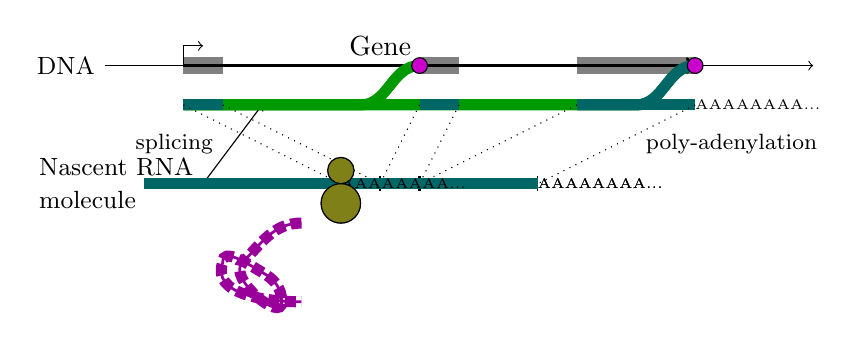
\begin{tikzpicture}[scale=0.5]
%    \draw [help lines] (0,0) grid (20,10);
    \draw [->, black!100] (1,9) -- (19,9);
    \visible<1-1>{ \node [left] at (1,9) {\small DNA}; }
    \uncover<2->{
      \draw[black!50, line width=6] (3,9) -- (4,9);
      \draw[black!50, line width=6] (9,9) -- (10,9);
      \draw[black!50, line width=6] (13,9) -- (16,9);
      \draw[->] (3,9) -- (3,9.5) -- (3.5,9.5);
      \draw[->,line width=1.2] (3,9) -- (16,9);
      \node [above] at (8,9) {Gene};
    }
    
    \visible<3>{
      \draw[rnaColor, line width=4] (3,8) -- (7.5,8) 
      to [out=0, in=180] (9,9);
      \draw[cdsColor, line width=4] (3,8) -- (4,8);
      \draw[<-] (5,8) -- (3.5,6) node[left, align=left] {\small Nascent RNA\\\small molecule};
      \draw [fill=rnaPol] (9,9) circle [radius=0.2];
    }

    \visible<4>{
      \draw[rnaColor, line width=4] (3,8) -- (14.5,8) 
      to [out=0, in=180] (16,9);
      \draw[cdsColor, line width=4] (3,8) -- (4,8);
      \draw[cdsColor, line width=4] (9,8) -- (10,8);
      \draw[cdsColor, line width=4] (13,8) -- (14.5,8)
      to [out=0, in=180] (16,9);
      \draw [fill=rnaPol] (16,9) circle [radius=0.2];
    }

    \visible<5>{
      \draw[rnaColor, line width=4] (3,8) -- (16,8);
      \draw[cdsColor, line width=4] (3,8) -- (4,8);
      \draw[cdsColor, line width=4] (9,8) -- (10,8);
      \draw[cdsColor, line width=4] (13,8) -- (16,8);
      \node[right] at (15.75,8) {\tiny AAAAAAAA...};
      
      \draw[cdsColor, line width=4] (7,6) -- (12,6);
      \draw[|-|] (7,6) -- (8,6);
      \draw[|-|] (8,6) -- (9,6);
      \draw[|-|] (9,6) -- (12,6);
      \node[right] at (11.75,6) {\tiny AAAAAAAA...};
      
      \draw [dotted] (3,8) -- (7,6);
      \draw [dotted] (4,8) -- (8,6);
      \draw [dotted] (9,8) -- (8,6);
      \draw [dotted] (10,8) -- (9,6);
      \draw [dotted] (13,8) -- (9,6);
      \draw [dotted] (16,8) -- (12,6);
      
      \node [left, align=left, font=\footnotesize] at (4,7) {splicing};
      \node [right, font=\footnotesize] at (14.5,7) {poly-adenylation};
    }

    \visible<6>{
      \draw[cdsColor, line width=4] (7,6) -- (12,6);
      \node[right] at (11.75,6) {\tiny AAAAAAAA...};
      \riboS[0.5]{7}{6};
    }

    \visible<7>{
      \draw[cdsColor, line width=4] (2,6) -- (7,6);
      \node[right] at (6.75,6) {\tiny AAAAAAAA...};
      \protein{6}{5};
      \riboS[0.5]{7}{6};
    }
  \end{tikzpicture}
  \end{figure}
\end{frame}

\begin{frame}{Eukaryotes \& Prokaryotes}
  \begin{columns}
    \begin{column}[T]{0.5\textwidth}
      \subHeading{Eukaryotes}
      \begin{itemize}
      \item One transcript containing introns and exons
      \item Introns removed and exons combined by splicing
      \item Enzymatic (non-template) addition of As at 3' end
      \item One protein produced
      \end{itemize}
    \end{column}
    \begin{column}[T]{0.5\textwidth}
      \subHeading{Prokaryotes}
      \begin{itemize}
        \item One transcript containing several open reading frames
        \item Each open reading frame translated seperately
        \item Several proteins produced
      \end{itemize}
    \end{column}
  \end{columns}
  \vspace{4ex}
  \visible<2->{
    \begin{itemize}
    \item Some polycistronic messages identified in eukaryotes.
    \item Introns can be found in prokaryotes (but \emph{very rare})
    \end{itemize}
  }
\end{frame}

\begin{frame}{Strandedness!!}
  \begin{figure}[ht]
    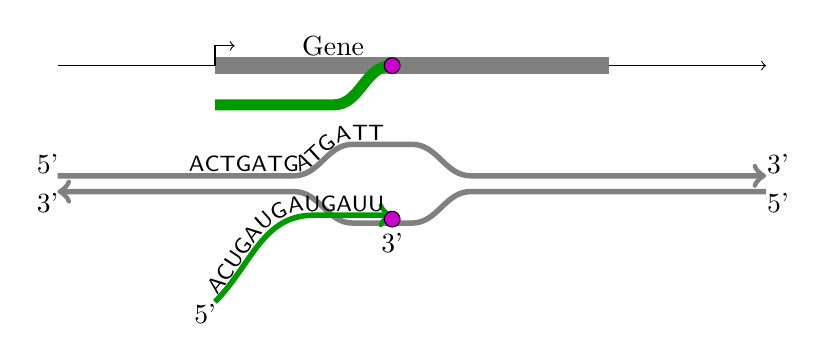
\begin{tikzpicture}[scale=0.5]
%%      \draw [help lines] (0,0) grid (20,10);
      \visible<1->{
        \draw [->, black!100] (1,9) -- (19,9);
        %%      \visible<1-1>{ \node [left] at (1,9) {\small DNA}; }
        %%     \uncover<2->{
        \draw[black!50, line width=6] (5,9) -- (15,9);
        \draw[->] (5,9) -- (5,9.5) -- (5.5,9.5);
        \node [above] at (8,9) {Gene};
        %%      }
        %%     \visible<3->{
        \draw[rnaColor, line width=4] (5,8) -- (8,8) 
        to [out=0, in=180] (9.5,9);
        \draw [fill=rnaPol] (9.5,9) circle [radius=0.2];
      }
 %%     }
      \visible<2->{
        \draw[black!50, line width=2,->] (1,6.2) -- (7,6.2)
        to [out=0,in=180] (8.5,7) -- (10,7) to [out=0,in=180] (11.5,6.2) -- (19,6.2);
        \draw[black!50, line width=2,<-] (1,5.8) -- (7,5.8)
        to [out=0,in=180] (8.5,5) -- (10,5) to [out=0,in=180] (11.5,5.8) -- (19,5.8);
        \draw[rnaColor, line width=2, <-] (9.5, 5.2) -- (7.5,5.2) to [out=180,in=45] (5,3);
        \draw[fill=rnaPol] (9.5, 5.1) circle [radius=0.2];
      }
      \visible<3->{
        \node at (0.75,6.5) {5'};
        \node at (19.3,6.5) {3'};
        \node at (0.75,5.5) {3'};
        \node at (19.3,5.5) {5'};
      }
      \visible<4->{
        \node at (4.75,2.7) {5'};
        \node at (9.5, 4.5) {3'};
      }
      \visible<5->{
        \draw [line width=0,black!0, draw=none,
          postaction={decorate,decoration={text along path,
              text align=right,text={|\fontsize{8}{10}\sffamily|ACTGATGATGATT}}}] 
        (4.5,6.3) -- (7,6.3)
        to [out=0,in=180] (8.5,7.1) -- (9.3,7.1); %% to [out=0,in=180] (11.5,6.3)
        -- (12,6.3);
      }
      \visible<6->{
        \draw [line width=0, black!0, draw=none,
          postaction={decorate,decoration={text along path,
              text align=right,text={|\fontsize{8}{10}\sffamily|ACUGAUGAUGAUU}}}] 
        (4.9,3) to [out=45,in=180] (7.4,5.3) -- (9.3,5.3);

%%        \draw [line width=0, black!50, 
%%          postaction={decorate,decoration={text along path, 
 %%             text align=left,text={|\fontsize{8}{10}|\sffamily|UAGUAGUAGUCA}}}] (9.5, 5.2) -- (7.5,5.2) to [out=180,in=45] (5,3);
      }
    \end{tikzpicture}
  \end{figure}
  
\end{frame}

\begin{frame}{Encoding of Amino Acid sequence in DNA}
  Four nucleotides $\Rightarrow$  20 Amino Acids\\Word length?
  \begin{itemize}
    \item $1 \rightarrow 4^1 = 4 $\\
      A, C, G, U
      \pause
    \item $2 \rightarrow 4^2 = 16$\\
      AA, AC, AG, AU, CA, CC, CG, CU, GA, GC, GG, GU, UA, UC, UG, UU, 
      \pause
    \item $3 \rightarrow 4^3 = 64$\\
      AAA, AAC, AAG, AAU, ACA, ACC, ACG, ACU, AGA, AGC, AGG, AGU, ...
  \end{itemize}
  \pause
  $\rightarrow$ triplet code used.
\end{frame}

\begin{frame}{Encoding of Amino Acid sequence in DNA (2)}
  \subHeading{Summary}
  \begin{itemize}
    \item Amino acid encoded by codons that contain 3 nucleotides each.
    \item 61 codons $\rightarrow$ 20 amino acids
    \item 3 codons $\rightarrow$ STOP
    \item 1 codon $\rightarrow$ START (AUG encodes Met)
  \end{itemize}
  \tiny Slightly simplified, but generally good enough.
\end{frame}

\begin{frame}{The \emph{standard} code}
\begin{figure}[ht]
  \tiny
  \renewcommand{\arraystretch}{1.25}
  \begin{tabular}{ |l| l l|l l| l l|l l|l| }
    \hline
    \multirow{2}{2em}{1st base} &
    \multicolumn{8}{|c|}{2nd base} &
    \multirow{2}{2em}{3rd base} \\
    \cline{2-9}
    &
    \multicolumn{2}{|c|}{U} &
    \multicolumn{2}{|c|}{C} &
    \multicolumn{2}{|c|}{A} &
    \multicolumn{2}{|c|}{G} & \\
    \hline
    \multirow{4}{2em}{U} & 
    UUU & \multirow{2}{4em}{\tiny (Phe/F)} &
    UCU & \multirow{4}{4em}{\tiny (Ser/S)} &
    UAU & \multirow{2}{4em}{\tiny (Tyr/Y)} &
    UGU & \multirow{2}{4em}{\tiny (Cys/C)} & U \\
    & UUC & & UCC & & UAC & & UGC & & C \\ \cline{2-3} \cline{6-9}
    & UUA & \multirow{6}{4em}{\tiny (Leu/L)} 
    & UCA & & UUA & Stop & UGA & (Stop) & A \\ \cline{8-9}
    & UUG & & UCG & & UAG & Stop & UGG & \tiny (Trp/W) & G \\ \cline{4-9} 
    \cline{1-1}
    \multirow{4}{2em}{C}
    & CUU & & CCU & \multirow{4}{4em}{(Pro/P)} & CAU & \multirow{2}{4em}{(His/H)} & CGU & \multirow{4}{4em}{(Arg/R)} & U \\
    & CUC & & CCC & & CAC & & CGC & & C \\ \cline{6-7}
    & CUA & & CCA & & CAA & \multirow{2}{4em}{Gln/Q} & CGA & & A \\
    & CUG & & CCG & & CAG & & CGG & & G \\ \cline{1-9}
    \multirow{4}{2em}{A}
    & AUU & \multirow{3}{4em}{(Ile/I)} & ACU & \multirow{4}{4em}{(Thr/T)} & AAU 
    & \multirow{2}{4em}{(Asn/N)} & AGU & \multirow{2}{4em}{(Ser/S)} & U \\
    & AUC & & ACC & & AAC & & AGC & & C \\ \cline{6-9}
    & AUA & & ACA & & AAA & \multirow{2}{4em}{(Lys/K)} & AGA & \multirow{2}{4em}{(Arg/R)} & A \\
    \cline{2-3}
    & AUG & (Met/M) & ACG & & AAG & & AGG & & G \\ \cline{1-9}
    \multirow{4}{4em}{G}
    & GUU & \multirow{4}{4em}{(Val/V)} & GCU & \multirow{4}{4em}{(Ala/A)} 
    & GAU & \multirow{2}{4em}{(Asp/D)} & GGU & \multirow{4}{4em}{(Gly/G)} & U \\
    & GUC & & GCC & & GAC & & GGC & & C \\ \cline{6-7}
    & GUA & & GCA & & GAA & \multirow{2}{4em}{(Glu/E)} & GGA & & A \\
    & GUG & & GCG & & GAG & & GGG & & G \\ \hline
  \end{tabular}
\end{figure}
\end{frame}

\begin{frame}{\emph{Non-standard} codes}
  \tiny
  \begin{description}[align=left]
    \item[1] The Standard Code
    \item[2] The Vertebrate Mitochondrial Code
    \item[3] The Yeast Mitochondrial Code
    \item[4] The Mold, Protozoan, and Coelenterate Mitochondrial Code and the Mycoplasma/Spiroplasma Code
    \item[5] The Invertebrate Mitochondrial Code
    \item[6] The Ciliate, Dasycladacean and Hexamita Nuclear Code
    \item[9] The Echinoderm and Flatworm Mitochondrial Code
    \item[10] The Euplotid Nuclear Code
    \item[11] The Bacterial, Archaeal and Plant Plastid Code
    \item[12] The Alternative Yeast Nuclear Code
    \item[13] The Ascidian Mitochondrial Code
    \item[14] The Alternative Flatworm Mitochondrial Code
    \item[16] Chlorophycean Mitochondrial Code
    \item[21] Trematode Mitochondrial Code
    \item[22] Scenedesmus obliquus Mitochondrial Code
    \item[23] Thraustochytrium Mitochondrial Code
    \item[24] Rhabdopleuridae Mitochondrial Code
    \item[25] Candidate Division SR1 and Gracilibacteria Code
    \item[26] Pachysolen tannophilus Nuclear Code
    \item[27] Karyorelict Nuclear Code
    \item[28] Condylostoma Nuclear Code
    \item[29] Mesodinium Nuclear Code
    \item[30] Peritrich Nuclear Code
    \item[31] Blastocrithidia Nuclear Code
    \item[33] Cephalodiscidae Mitochondrial UAA-Tyr Code
  \end{description}
\end{frame}

\begin{frame}[fragile]{Example codes}
  \begin{itemize}
  \item The standard code\\*
    \tiny
\begin{verbatim}
    AAs  = FFLLSSSSYY**CC*WLLLLPPPPHHQQRRRRIIIMTTTTNNKKSSRRVVVVAAAADDEEGGGG
  Starts = ---M------**--*----M---------------M----------------------------
  Base1  = TTTTTTTTTTTTTTTTCCCCCCCCCCCCCCCCAAAAAAAAAAAAAAAAGGGGGGGGGGGGGGGG
  Base2  = TTTTCCCCAAAAGGGGTTTTCCCCAAAAGGGGTTTTCCCCAAAAGGGGTTTTCCCCAAAAGGGG
  Base3  = TCAGTCAGTCAGTCAGTCAGTCAGTCAGTCAGTCAGTCAGTCAGTCAGTCAGTCAGTCAGTCAG
\end{verbatim}
\normalsize
\item The vertebrate mitochondrial code\\*
  \tiny
\begin{verbatim}
    AAs  = FFLLSSSSYY**CCWWLLLLPPPPHHQQRRRRIIMMTTTTNNKKSS**VVVVAAAADDEEGGGG
  Starts = ----------**--------------------MMMM----------**---M------------
  Base1  = TTTTTTTTTTTTTTTTCCCCCCCCCCCCCCCCAAAAAAAAAAAAAAAAGGGGGGGGGGGGGGGG
  Base2  = TTTTCCCCAAAAGGGGTTTTCCCCAAAAGGGGTTTTCCCCAAAAGGGGTTTTCCCCAAAAGGGG
  Base3  = TCAGTCAGTCAGTCAGTCAGTCAGTCAGTCAGTCAGTCAGTCAGTCAGTCAGTCAGTCAGTCAG
\end{verbatim}

\normalsize
\item The yeast mitochondrial code\\*
  \tiny
\begin{verbatim}
    AAs  = FFLLSSSSYY**CCWWTTTTPPPPHHQQRRRRIIMMTTTTNNKKSSRRVVVVAAAADDEEGGGG
  Starts = ----------**----------------------MM---------------M------------
  Base1  = TTTTTTTTTTTTTTTTCCCCCCCCCCCCCCCCAAAAAAAAAAAAAAAAGGGGGGGGGGGGGGGG
  Base2  = TTTTCCCCAAAAGGGGTTTTCCCCAAAAGGGGTTTTCCCCAAAAGGGGTTTTCCCCAAAAGGGG
  Base3  = TCAGTCAGTCAGTCAGTCAGTCAGTCAGTCAGTCAGTCAGTCAGTCAGTCAGTCAGTCAGTCAG
\end{verbatim}
  \end{itemize}

  \footnotetext[1]{\tiny
  https://www.ncbi.nlm.nih.gov/Taxonomy/Utils/wprintgc.cgi }
\end{frame}

\begin{frame}[fragile]{Reading frames}
  \begin{figure}[ht]
    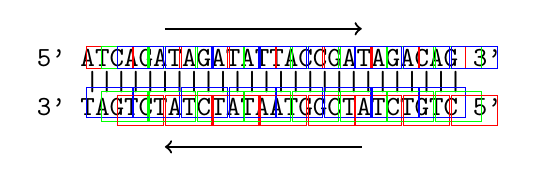
\begin{tikzpicture}[scale=0.5]
%      \draw [help lines] (0,0) grid(20,5);
      \visible<3-5>{
        \draw [->,thick] (7.5,4.75) -- (12.5,4.75); 
      }
      \visible<6->{
        \draw [<-,thick] (7.5,1.75) -- (12.5,1.75); 
      }
      \node[right, font=\ttfamily, align=left] at (4,4) 
           {5' ATCAGATAGATATTACCGATAGACAG 3'};
      \visible<2->{
        \node[right, font=\ttfamily, align=left] at (5.225,3.4)
             {||||||||||||||||||||||||||};
             \node[right, font=\ttfamily, align=left] at (4,2.75)
                  {3' TAGTCTATCTATAATGGCTATCTGTC 5'};
      }
      \visible<3>{
        \foreach \x in {5.5, 6.71,...,15} {
          \draw [red] (\x, 3.75) rectangle (\x + 1.17, 4.3);
        }
      }
      \visible<4>{
        \foreach \x in {5.9, 7.11,...,15.5}{
          \draw [green] (\x, 3.75) rectangle (\x + 1.17, 4.3);
        }
      }
      \visible<5>{
        \foreach \x in {6.3, 7.51,...,15.5}{
          \draw [blue] (\x, 3.75) rectangle (\x + 1.17, 4.3);
        }
      }
      \visible<6>{
        \foreach \x in {5.5, 6.71,...,15} {
          \draw [blue] (\x, 3.75-1.25) rectangle (\x + 1.17, 4.3-1.05);
          \draw [green] (\x + 0.4, 3.75-1.35) rectangle (\x + 1.17 + 0.4, 4.3-1.15);
          \draw [red] (\x + 0.8, 3.75-1.45) rectangle (\x + 1.17 + 0.8, 4.3-1.25);
        }
      }
    \end{tikzpicture}
  \end{figure}
  This can encode amino acids in 6 different ways:
{
  \small
  \begin{description}
    \item<3->[frame 1]
      \begin{verbatim}
.. ATC AGA TAG ATA TTA CCG ATA GAC AG
   Ile Arg     Ile Leu Pro Ile Asp  \end{verbatim}
    \item<4->[frame 2]
      \begin{verbatim} 
.A TCA GAT AGA TAT TAC CGA TAG ACA G  
   Ser Asp Arg Tyr Tyr Arg     Thr
\end{verbatim}
    \item<5->[frame 3]
      \begin{verbatim}
AT CAG ATA GAT ATT ACC GAT AGA CAG 
   Gln Ile Asp Ile Thr Asp Arg His
\end{verbatim}
    \item<6->[frame -1]
      \begin{semiverbatim} .. CTG TCT ATC GGT AAT ATC TAT CTG AT \end{semiverbatim}
    \item<6->[frame -2]
      \begin{semiverbatim} .C TGT CTA TCG GTA ATA TCT ATC TGA T \end{semiverbatim}
    \item<6->[frame -3]
      \begin{semiverbatim} CT GTC TAT CGG TAA TAT CTA TCT GAT .. \end{semiverbatim}
  \end{description}
}
\end{frame}

\begin{frame}{Reading frames (2)}
  DNA is\footnote{Well in general anyway. It can be single stranded as well,
    but then you'll usually be informed.}
  double stranded and has 6 reading frames.
  \vspace{3ex}

  RNA is single stranded\footnote{Well, it can be double-stranded as well, but...}; it has only 3 reading frames!
\end{frame}

\begin{frame}{Open Reading Frame (ORF)}
  \begin{itemize}
    \item Refers to a stretch of codons (nucleotide triplets) in the same frame that
      do not contain any stop codons (UUA, UAG, UGA).
    \item Sometimes required to begin with a start codon (AUG), but this depends on circumstance.
    \item Long ORFs indicate the presence of protein coding genes.
  \end{itemize}
\end{frame}

\begin{frame}{Frames and mutations}
    \begin{columns}
      \begin{column}{0.5\textwidth}
        4 types of mutations
        \begin{itemize}
          \item substitution
          \item insertion
          \item deletion
          \item recombination events
        \end{itemize}
      \end{column}
      \begin{column}{0.5\textwidth}
        ORF effects
        \begin{itemize}
          \item amino acid change (?)
          \item frame shift
          \item frame shift
          \item complex change
        \end{itemize}
      \end{column}
    \end{columns}
\end{frame}

\begin{frame}{Summary}
  \begin{figure}[ht]
    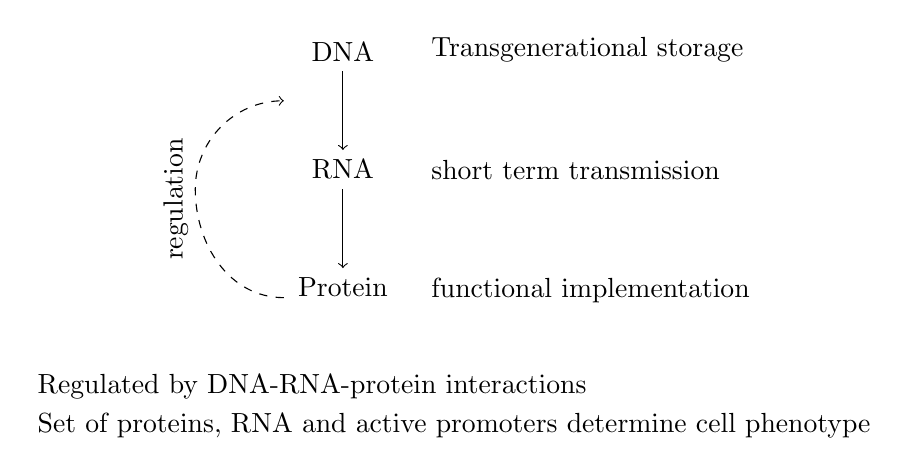
\begin{tikzpicture}[scale=0.5]
      \draw [help lines, opacity=0] (0,0) grid(20,10);
      \node [above] at (8,9) {DNA};
      \node [above right] at (10,9) {Transgenerational storage};
      \draw [->] (8,9) -- (8,7) node [below] {RNA};
      \node [below right] at (10,7) {short term transmission};
      \draw [->] (8,6) -- (8,4) node [below] {Protein};
      \node [below right] at (10,4) {functional implementation};
      \draw [->, dashed] (6.5,3.25) to [out=180,in=270] (4.25,6)
      to [out=90,in=180] (6.5,8.25);
      \node [rotate=90] at (3.75,5.75) {regulation};
      \node [right] at (0,1) {Regulated by DNA-RNA-protein interactions};
      \node [right] at (0,0) {Set of proteins, RNA and active promoters determine cell phenotype};
    \end{tikzpicture}
  \end{figure}
\end{frame}

\end{document}
